\chapter{2. Background and Motivation}

\begin{quote}
\textit{If I had an hour to solve a problem and my life depended on it, I'd spend the first 55 minutes determining the proper question to ask. \newline\begin{flushright}- Albert Einstein\end{flushright}} \newline
\end{quote}
\newline

There are many issues standing in the way of low-cost, portable, and effective air quality measurement.  While the field is ripe for innovation, a thorough understanding of the state-of-the-art (and its limiting factors) is important before attempting to make progress.  The following section represents months of distilled advice from industry experts and thought leaders, who greatly informed the direction of this work.  

\section{Air Monitoring}

\subsection{Air Pollutants}

Despite the complexities of behind sparce air quality measurement and individual health, there is a plethora of evidence linking small particulate matter and other pollutants to serious negative health effects.

Particulate matter is designated according to its size-- PM2.5 are particles with 2.5 micron diameter or less, PM10 has a 10 micron diameter or less, and ultrafine particulate (UFP) are measured in nanometers (equivalent to PM1).  These designations are made based on human physiology.  Particles larger than 10 microns are typically filtered in the nose and throat; below this size, the particles are considered 'respirable'.  Particles between 10 and 2.5 microns can usually penetrate into the lungs and settle, while particles less than 2.5 microns tend to pass into the alveoli and into the bloodstream.  Nanoparticles are so small that some can pass through cell membranes, and damage other organs throughout the body.  Additionally, particulate deposition is different for these groups-- PM10 may settle out of the air in hours, while the smaller and lighter particles generally stay in the air until there is precipitation.

Particulate size distribution is generally viewed as the sum of \textit{n} log-normal distributions.  Nucleation by-products from engine combustion drives a positively-skewed, log-normal distribution centered at a few hundred nanometers.  Mechanically generated road dust on paved and unpaved roads generates a negatively-skewed log-normal particle distributions favoring 10 micron diameters.  Pollen also has a negatively skewed log-normal distribution in the 10-100 micron range.  The greatest health risk is associated with the smallest diameter (often nucleation-based) particulate.  

Specific gases have also been linked to health risk, and the United States Environmental Protection Agency (EPA) has set standards for five other pollutants-- Lead, Nitrogen Oxides, Carbon Monoxide, Sulfer Dioxide, and Ozone.

The main sources of lead exposure (automotive fuel and paint) have been heavily regulated over the past several decades in first world countries.  The last industrial lead smelter in the United States shut down two years ago, and airborne lead exposure in the first world is almost a mute point outside of old house paint.  Airborne lead is still an issue in developing countries, however, especially near unregulated smelters that recycle car batteries.

The result of incomplete or high temperature automotive combustion, Nitrogen Oxides and Carbon Monoxide (as well as Black Carbon, a major constituent of PM2.5) are common pollutants in the urban setting.  Since the sources of these pollutants are mobile, they often manifest with complex spatiotemporal dynamics, including temporary hotspots of high exposure.

Sulfur Dioxide is the result of fossil fuel combustion, and is thus detectable near power plants and other industrial operations. 
  
Ozone at the earth's surface is typically the result of Volatile Organic Compounds (VOCs) reacting with Nitrogen Oxides in the presence of sunlight.  Thus, while vehicle emissions seed the process, ozone concentrations tend to be dependent on sunlight, and therefore more predictable and less dynamic than CO, NO2, and PM.

EPA standards are set at 75 ppb average per hour for SO2, 100 ppb average per hour for NO2, 70 ppb average for 8 hours for Ozone, 9 ppm average for 8 hours for CO, and annual averages of 0.15 \(\mu g/m^3\) for Pb, 12 \(\mu g/m^3\) for PM2.5, and 35 \(\mu g/m^3\) for PM10.

\subsection{Sensor Technologies for Particulate Matter}

\begin{marginfigure}[3.5cm]
 	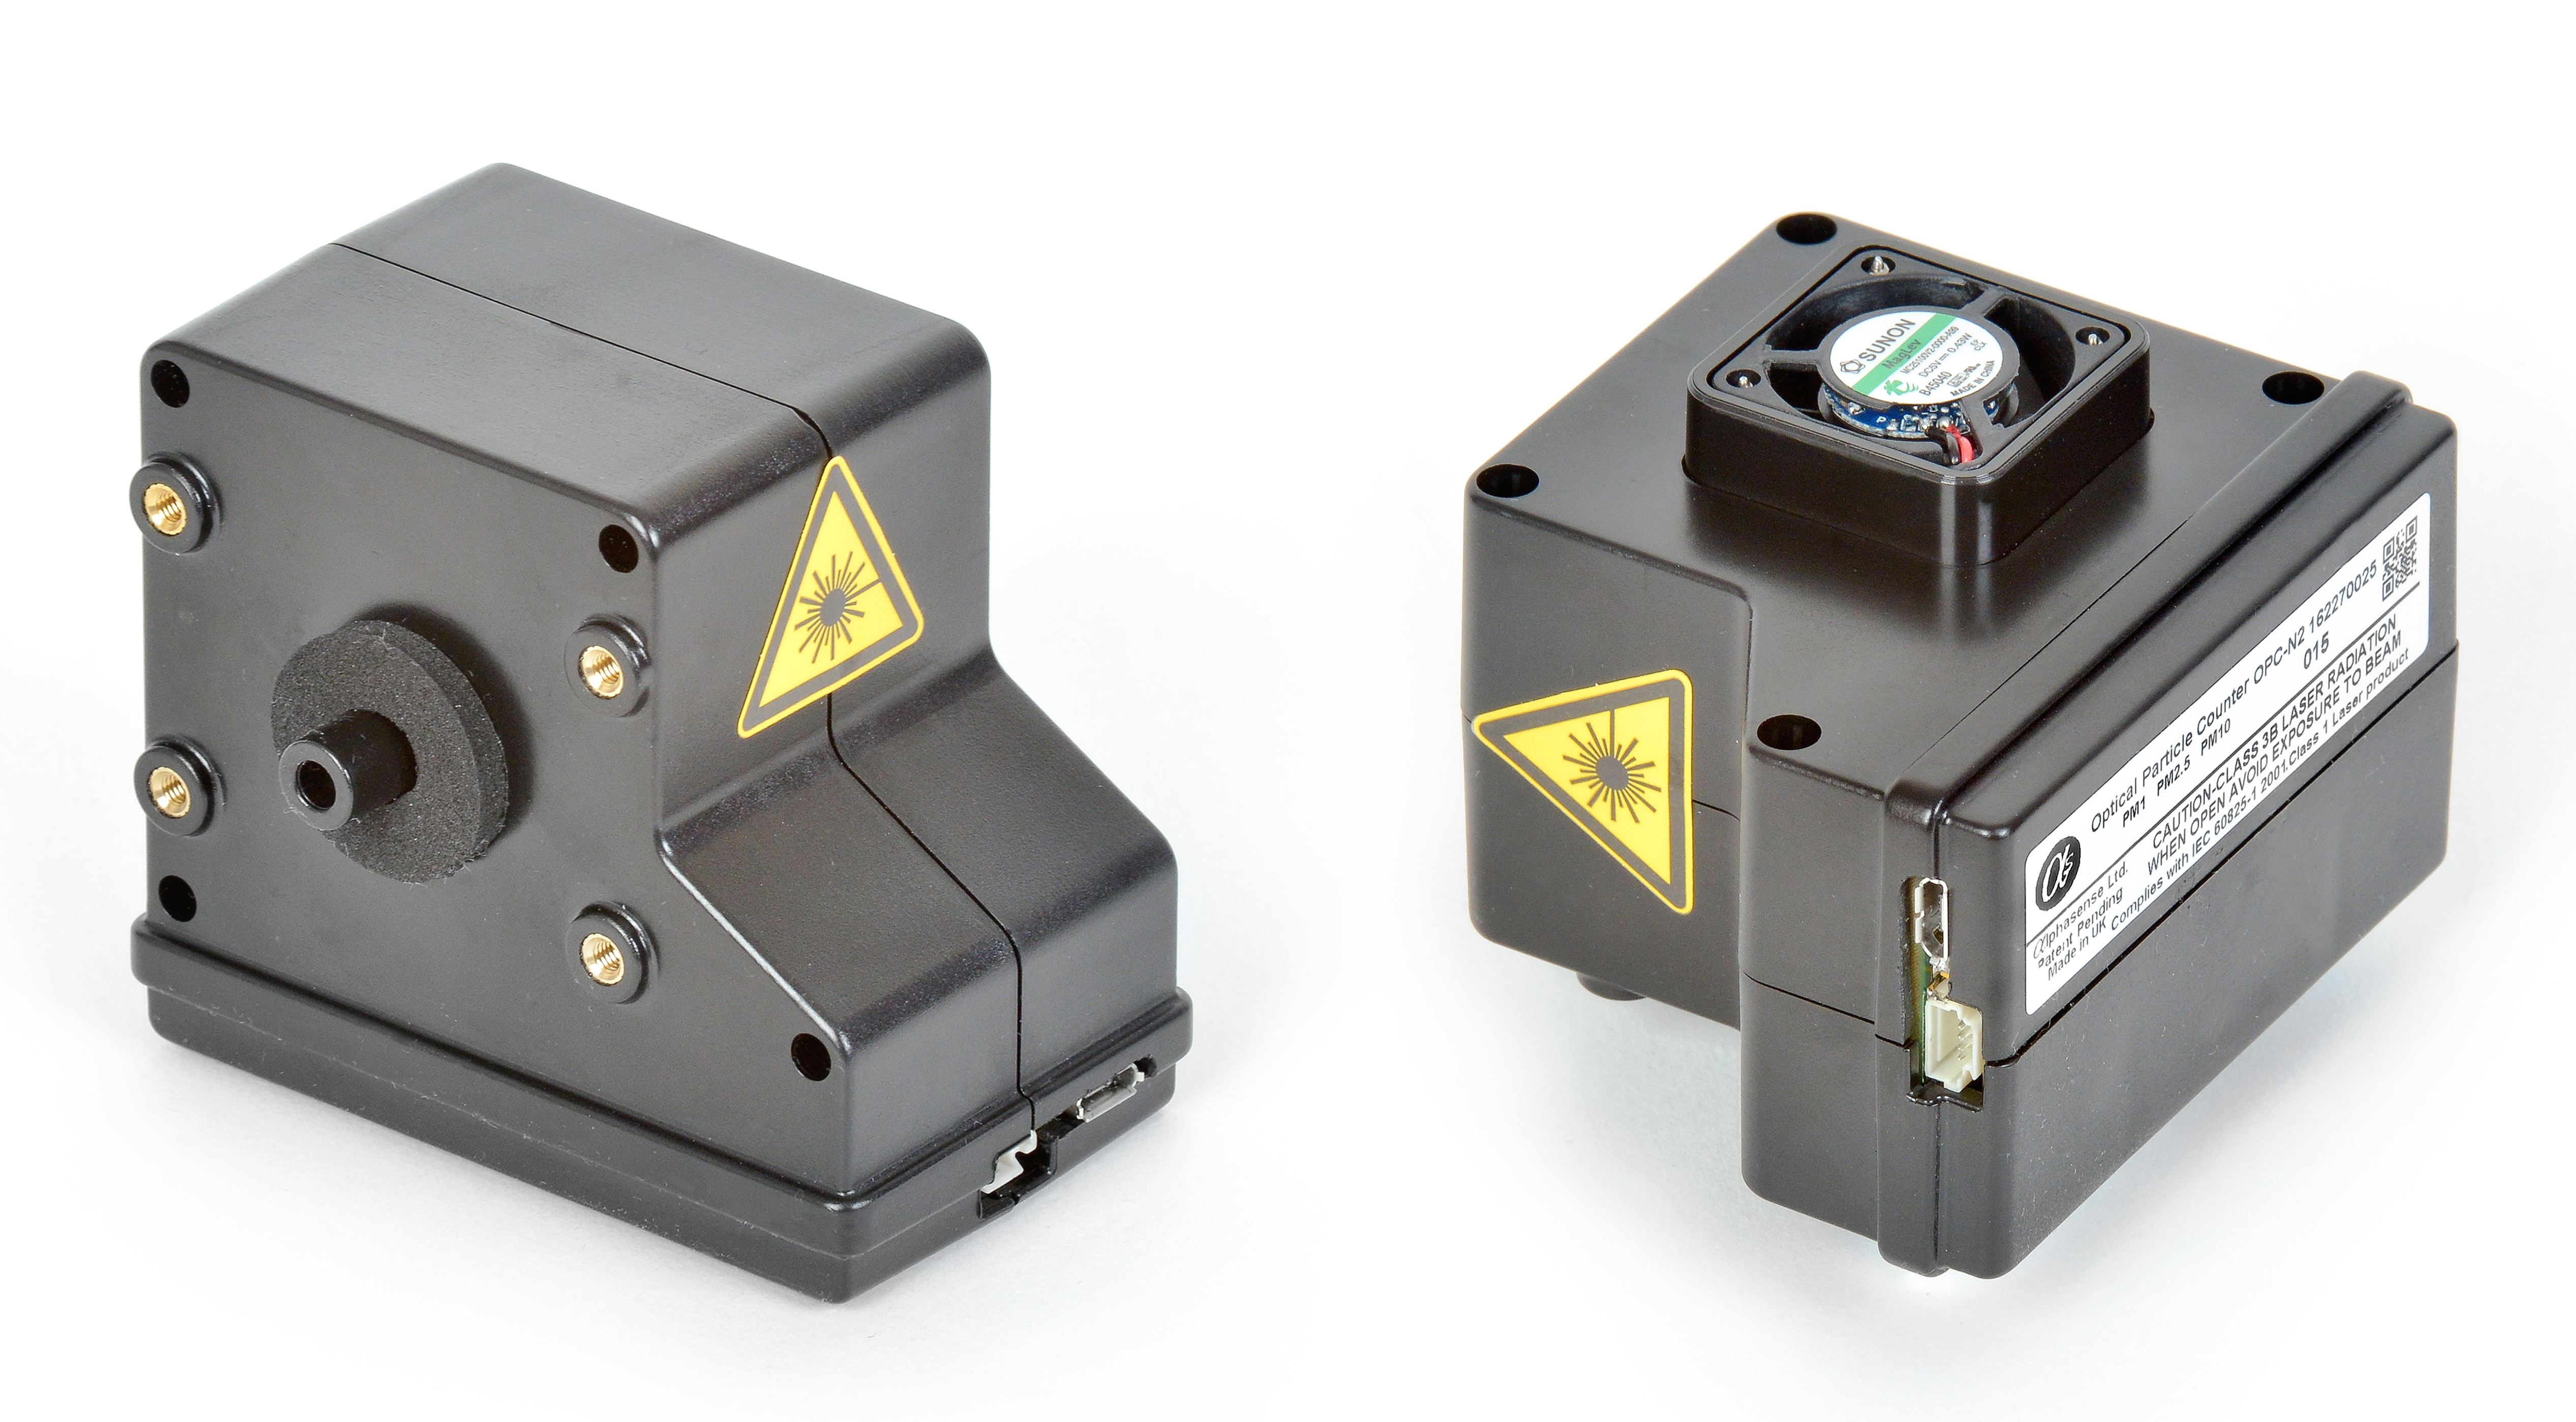
\includegraphics[width=\textwidth]{visuals/as_optical}               
 	 \caption{AlphaSense Opitcal PM2.5 Sensors.}
  	\label{fig:as_optical}
\end{marginfigure}

There are many sensor modalities for pollution monitoring, with a handful separating themselves as the standard references.  For particulate, high quality, large installations will usually either have a Beta Attenuation Monitor (BAM) or a Tapered Element Oscillating Microbalance (TEOM) sensor for particulate sensing.  BAM sensors collect particulate on successive circular sections of a long filter that is spooled inside the device.  Measurements are taken by simply analyzing the beta particle attenuation through the filter.  TEOM sensors draw air through a filter so particulate deposits on the end of an oscillating cantilever (its resonant frequency is dependent on its mass).  The more mass is deposited on the filter, the lower the resonant frequency, which is measured and used to calculate very accurate particulate levels.  Other methods typically include gravimetric techniques with filters that are analyzed in a lab environment.

Optical methods for particulate sensing are particularly important in the mobile context.  Since particulates are measured in \(\mu g/m^3\), their accuracy depends on assumptions about airflow through the device, as well as the assumed statistics of particle size and mass distributions (which can change from location to location depending on the local mixture of pollutants).  

Optical PM sensors typically have similar geometry- a narrowly focused IR beam is broken by the particles, and the scattered light is measured by an off-angle photodiode.  For cheap sensors, airflow through the device is not tightly controlled (it may be driven by convection with a small heating element, but it is never precise), the optics are coarse, and the captured light is only a loose representation of particulate level.  Better sensors use a more tightly focused beam, as well as a fan to control airflow, and can simply count pulses as the beam breaks-- with a known, precisely controlled airflow, the length of time the beam is broken is proportional to particle size.  The final and best type of optical technique uses Mie Scattering, which calculates particle size by looking at intensity of the scattered light on the photodiode (a nonlinear monotonic function with particle size). In this way the duration of a particle in front of the beam can be used independently to verify flow rate, and address small errors in its control.  In all of these designs, larger particles have a non-trivial deposition rate, which further constrains the geometry and flow through a device.   Expensive optical variants include Condensation Particle Counters, in which particle size is increased in a predictable way by condensing vapor from a working fluid around the particles, making them easier to count. Electrical mobility sorting based on size/charge of particle in electrostatic field is also sometimes used in concert with optical techniques.

Inlets are included on all professional level equipment.  These inlets protect the device from wind, create predictable airflow, and typically include particle size selectivity.  Most commonly, size selectivity is achieved using inertial techniques (i.e. impaction or cyclone filtering).  They are generally mounted in an upright position due to particle deposition (so gravity works with the inlet), and they are sometimes heated to evaporate fog.

For cheap, small, or mobile applications, optical sensing has been the dominant modality.  On the high end (>\$15k), handheld systems like the Grimm Enviro 11E have nice inlet and size selectivity, advanced optics, and create sheathing airflow out of filtered air, which helps collimate incoming samples and clean the beam path.  These professional quality systems have been used in research studies to evaluate personal exposure, but they clearly do not offer a viable option for distributed or personal applications.  

On the cheaper end of the spectrum, many sensors exist.  Unfortunately, independent tests have shown that none of these hold up in dynamic, real-world situations. One in particular worth noting is the Shinyei PPD42NS, a \$10 sensor that is widely used and cited as providing high quality results. It has a small heating element for inducing convective flow, and coarse optics.  Unfortunately, its reputation is based on very controlled conditions.  In outdoor tests, the Shinyei provided erroneous results, demonstrating enormous cross-sensitivity to variations in airflow, temperature, and humidity. The lack of clarity around the useful application space of cheap optical sensors is an unfortunate common misconception, and demonstrates the importance of testing these sensors in realistic mobile contexts.

The \$300 Dylos seems to be the cheapest optical sensor that stands up reasonably well in independent tests. It uses an IR laser and has a much larger and more sophisticated flow design than its cheaper counterparts.

The \$400 OPC-N2 is an optical particle sensor similar to the Dylos, but much smaller.  It uses a fan to drive a fixed flow rate, and take advantage of Mie Scattering principles to correct for variations in flow rate through the device.  AlphaSense has not released a full characterization of their design, but preliminary testing in environmental sensing groups at MIT have yielded mixed results-- it appears that the OPC-N2 is incapable of sensing particles below a few hundred nm in diameter, which make up most of the mass concentration of PM2.5.  

Since PM2.5 mass is largely made up of nucleation/combustion driven particulate, its core component follows a log-normal size distribution centered in the nm range.  While measuring the log tail can provide some insight into the core of the distribution, tails from larger particulate like mechanically-created road dust or pollen (mostly 10-100micron) overlap in the critical 300nm-10micron range where the OPC-N2 is sensitive.  This presents serious challenges infering a relationship between what is actually measured in the 300nm-10micron range and PM2.5 levels without extra information.  

\subsection{Sensor Technologies for Gas Sensing}

\begin{marginfigure}[3.5cm]
 	\includegraphics[width=\textwidth]{visuals/as_gas}               
 	 \caption{AlphaSense Electrochemical Gas Sensors.}
  	\label{fig:as_gas}
\end{marginfigure}

For sensing specific gases, many types of sensors are used.  Among other techniques, spectroscopy, chromatography, and chemiluminescence are very common for professional applications.  For mobile use, Alphasense sensors have emerged with a strong cost to performance ratio.  Alphasense sells Photoionization Detection based sensors, which work by ionizing gas particles with UV light and sensing the generated current over a fixed voltage in contact with the air. They also sell Nondispersive IR sensors, a simple optical absorption method.  

For the specific types of gases we're interested in, electrochemical techniques are the primary low cost method on the market.  The AlphaSense version is well-regarded, with ppb sensitivities and a clear failure condition (instead of the gradual drift you might expect as the sensor is depleted and dirtied). Electrochemical gas sensors are comprised of a working electrode, a reference electrode, and a counter electrode, all bathed in an electrolyte.  The reference electrode is used to control the voltage at the working electrode, and keep it in a linear current/voltage regime.  The working and counter electrodes promote inverse oxidation/reduction reactions, combining with the gas to produce free electrons, and then balancing that first reaction so as not to deplete or change the available reactants. The resulting current is proportional to the gas concentration, as long as corrections are applied for temperature, humidity, and pressure (and adequate time is allowed for 'warming up' once the reference electrode is powered on due to large inter-electrode capacitance).  These sensors are generally well-characterized under stable operating conditions, and have well understood cross-sensitivities and time-constants associated with their behavior.

While AlphaSense sensors can be purchased with calibration data, environmental sensing researchers at MIT have suggested that these calibrations are generally not accurate, and typically co-locate the sensors with a Federal Reference sensor for more rigorous calibration before deploying them elsewhere. 

\subsection{Measurement Strategies and Complications}

Historically, the standard measure of air quality has been a sparse network of fixed stations run by government agencies.  These extremely expensive and extremely large stations require manual calibration every few weeks.
	
While these stations are highly accurate, studies have shown they either chronically underreport or have no correlation with the personal exposure of the citizens living near them. Only with sophisticated modeling of elevation, geography, ambient conditions, wind velocity, and land use can these data be tied to exposure elsewhere in a city, and these models must be evaluated on a case-by-case and pollutant-by-pollutant basis.  
	
New techniques to map and model a city using a small number of medium quality, mobile sensors have started to emerge. Stationary, high quality sensors play an important role in calibrating these systems on-the-fly, but these methods have shown much better predictive power for mapping cities in higher spatial resolutions.  However, their predictive power is still best on timescales of years and weeks, and starts to break down as they move towards days and hours.

Models on these timescales and resolutions are useful for understanding general trends in exposure for a city, as well as identifying and eliminating pollution sources, hotspots of high exposure, and issues with urban planning.  However, even these mobile techniques for map generation are limited in their ability to predict personal exposure.

Personal exposure is so difficult to measure because pollutant concentrations can vary dynamically.  For certain conditions researchers have modeled this complex behavior, and thanks to expensive portable sensors there have been several studies to corroborate their findings.  One common phenomenon is called the 'urban canyon'-- a street with two tall buildings on either side that creates several interacting, swirling vortices.

Measurements have shown CO and UFP concentrations doubling on one side of the street relative to the other in an urban canyon, measured at the same time of day. This variability has been demonstrated time and again-- one study showed complex relationships between different pollutants measured in the center of the street versus the sidewalk. Different corners of the same intersection can also vary tremendously. Even walking roadside vs. building-side on the same sidewalk has been linked to significant differences in pollution exposure level.

This is all to say that spatial variation is extremely high.  Concentrations can change drastically over just a few meters.  For true personal exposure monitoring, it is regarded as best practice to sample air within 30cm of the mouth and nose. While some of these spatial phenomena may fit an urban canyon model, and some may be modeled accurately with standard dispersion, few real-world scenarios are predictable with any single technique (especially to within a few meters).  It is extremely difficult to predict real spatial variation without direct measurement. 

Temporal variation is equally difficult to monitor. Studies at traffic intersections have shown that regular, tenfold increases in pollutant concentration occur over just one second. This staggering variation is averaged out even with the some of the best 'real-time' techniques-- fifteen second integration would miss the entire event.  Peak exposure levels may have important health implications, and in most cases transient events like this account for the majority of urban exposure.

Given the tremendous spatiotemporal variation in pollution, wearable air quality monitoring is clearly the only viable path to accurate personal exposure data.  Fixed and mobile sensors, even with state-of-the-art predictive resolution, can't capture the detail required to estimate individual exposure (especially considering the accepted standard of 30 cm from the mouth and nose for accuracy). 

With enough adoption, it is not difficult to image improving the collection and prediction of city-wide pollution mapping traditionally associated with fixed sensor installations.  Eventually, wearable sensor data may even enable accurate path-based personal exposure modeling (statistical relevance on the order of meters and minutes), since the data is collected from varied users in the real microenvironments that dominate their exposure.  Accounting for this otherwise highly specific spatiotemporal resolution would be difficult with any alternative method (day and 100m2 resolution is the best we see with predictive models right now).  As mobile sensing increases in accuracy and drops in cost, distributed sensing will usher in a new way of understanding the pollution landscape and our exposure to it.


\section{Sensor Networks}

\subsection{Air Quality Sensor Networks}

It is not uncommon to see publications describing cheap and portable smart-phone based air quality projects.  In most cases, these publications focus on system design, and produce thought-provoking work on the user-interface.  In cases where technologists explore new sensor design, it is rare they achieve compelling improvements.  The past 20 year has seen a lot of incremental optimization in the most promising sensing modalities.  Few research labs are positioned to push the state-of-the-art further by simply re-applying the same core physics without a fundamentally new insight.  Significant effort has brought us to current level of sophistication, and any incremental progress at the sensor level requires an equally sophisticated understanding.   

Outside of phone applications, true system-level research in the air quality space is uncommon.  Most air quality networks use the same topology-- one type of sensor device with standard, centralized data collection methods.  The exception to this rule comes out of ETH Zurich's OpenSense project, where mobile sensors check their calibration as they pass higher-quality fixed sensors.  OpenSense has also pioneered methods for multi-hop mobile sensor calibration.  Their work sets the standard for exploratory new air quality sensor network topologies.

In the consumer space, many projects and devices are launching on regular basis.  Unfortunately, most devices do not stand up to independent scrutiny, and rarely do they offer meaningful improvements over the status quo.  None of these devices has succeeded at sustaining momentum.  SmartCitizen is an example-- after a successful 2014 kickstarter with 600 backers and \$68k raised, the SmartCitizen online network currently shows no active devices (despite 618 having been registered).  The constant barrage of 'new' monitoring devices-- without accountability, without rigorous data-collection, and without real-world use-cases-- saturates and dilutes consumer response to these important issues.   

Citizens aren't the only ones purchasing air quality sensor devices.  Many cities are installing high-density pollution monitoring networks-- in some cases, only later realizing that the data is not of reasonable quality.  London (quite publicly) recently released a network of GPS-tracked, tweeting pidgeons with NO2 sensor backpacks-- while driven by a marketing firm as a (very successful) publicity campaign, it is a safe bet that data quality assurance is low.

The EPA publicly states that distributed, cheap sensing technology will be a cornerstone of their future success.  As part of the effort to engage with active citizens and communities, the EPA measures and publishes data about low cost consumer devices.  Currently this is done by co-locating the consumer device with a Federal Reference Measurement (FRM) device outside for several months (usually through a change of seasons).  This validation is not standardized or rigorously defined.  The end result is a simple regression comparison (produced by hand), and a single designation for the sensor (i.e. 'good' or 'bad').  Other organizations do similar co-location experiments (like SCAQMD), but no standard procedure has been agreed upon.

\subsection{Large Scale Data Sharing}

The air quality research community is actively looking for solutions to facilitate inter-organization data-sharing, so that large scale collaboration can become more commonplace.  They are also actively working to educate, involve, and benefit from the citizen sensing movement.  There are many open questions around how to structure an ecosystem with variable quality data, how to define data standards, and how data should be hosted. 
 
The most common solution for large-scale data sharing is to construct a centralized 'cloud' database with strict data standards and a strict ontology.  Generally, users prepare their data to meet the standard, and then push their data to the database using some basic tools.  As the most common structure, there are options that have library support for various file formats and hardware platforms.  Examples include data.sparkfun.com (which integrates directly with arduino shields) or plenar.io (which has easy csv upload and nice data selection/access features).  

\subsection{ChainAPI}

When it comes to robust solutions for large scale sensor networks that directly feed into a database, the possible options are less well-defined.  An ideal ecosystem would allow large scale networks to interact seamlessly, while still allowing freedom in ontology and distributed hosting (similar to the World Wide Web).  While there are several solutions starting to appear for Internet of Things applications (the so called 'Web of Things'), many are over-specified, and up until now the practical result has been for industry players to silo their hardware, their data, and their applications.  Industry consortia are starting to form to address these problems,  but the issues are still unresolved.

ChainAPI offers a thin, HAL- and JSON-based hypermedia solution for creating a distributed, browsable data resource.  It dictates enough structure to make resources easily linkable, new ontological relationships easily definable, and datasets easily accessible, searchable, and streamable.  It leaves open the questions of ontology and backend database structure. 

ChainAPI has been successfully used for a large-scale ecological installation in Southern Massachussetts.  It serves as the backbone for many interesting data visualizations, audio compositions, and future-looking tools.  It provides extensible answers to many questions facing the world of large scale, distributed sensor installations and their associated data.

\subsection{Machine Learning}

Machine learning provides a way to design algorithms that learn and improve as more data is provided.  These techniques have been applied to sensor data in a variety of forms.  Examples range from predicting the number of people in a closed space by looking at changes in distributed sensor readings (i.e. temperature, humidity, light, and pressure), to predicting soil moisture based on remote sensing techniques (i.e. vegetation index and light backscatter).  One notable research project used HVAC sensor data, both analytically and redundantly, to predict and verify whether other sensors in the network were working properly and automatically replace unreliable data.

Generally, all of these examples use supervised learning approaches with some form of cross-validation to validate success.  While each uses a different core algorithm (and there is room to test and apply all of them to the air quality space), one worth mentioning is the logistic regression.  Logistic regression is frequently used to predict engineering failure of products or systems.  It can be applied as a binary classifier (i.e., 'Is this sensor failing?'), as well as give a probability for each outcome ('yes' or 'no').
  

\section{Motivation}

Air pollution is a health risk for people around the world.  While standard measurement techniques are highly accurate, they are also extremely expensive and stationary.  These stationary sensors fall short of capturing meaningful information about a citizen's personal exposure-- the spatiotemporal variations of pollution concentration are too complex and too narrowly resolved to be captured with a single, distant sensor.

For exacting personal monitoring, wearable, mobile sensing is the only answer.  Sensors do exist that can measure personal exposure, but they are either thousands of dollars or they are cheap and inaccurate.  While elusive, portable, affordable sensing, has the potential to offer powerful insights for both individuals and research organizations.

The lack of cheap solutions is not due to a lack of understanding.  The core device physics of most sensors have been well-optimized over several decades, and the sophistication underlying their reference level counterparts is truly remarkable.  Cheap sensors are starting to mirror the core principles of instrument-grade devices.  Unforunately, there are systemic failures in cheap systems that simply are fundamental to the underlying sensor modality.  

Optical sensors, for instance, require precision optics, heated inlets, flow control, and size-selective filtration.  Solutions to these problems require extra power, extra size, or extra cost (and frequently all three).  Addressing these problems would push a cheap, portable sensor out of its category.  Electrochemical gas sensors require a clean, precision doping process, a statistically minimal exposed surface area, and compensation for fow rate, pressure, temperature, humidity, and electrical noise.  The physics limit how small they can be, and the market limits how much cost can be driven out of the manufacturing process.

There are two main take-aways from this survey-- the first is that attempting to incrementally improve devices by re-exploring their core physics is a difficult proposition.  The core physics are well-understood and companies have been optimizing them successfully for decades.  The first order problems with cheap sensors are \textit{not} with the core device principles, but with well-understood failure modes (like flow control, fog, temperature dependence, or chemical cross-sensitivity).  

The second take-away is that, excitingly, the core physics underlying cheap commercial sensors are approaching a very high quality.  This suggests that the sensors-- when they fail to provide accurate readings-- are likely doing so because of systemic, predictable failures.  If that was one single failure (like an optical sensor that is reliable except when fog is present), it would be trivial to predict when the sensor data is reliable based on fog measurements.  In real-world scenarios, however, multiple failure modes compound and obfuscate underlying robustness.

The belief that cheap sensors are now entering a quality regime where failure is more predictable leads us to machine learning as a potentially powerful mechanism to explore sensor performance and improve reliability.  Machine learning is perfectly suited to tease out these complicated underlying relationships.  Instead of the common approach of \textit{improving} sensor performance, the research suggests that \textit{characterizing} and \textit{predicting} sensor reliability in a nuanced way is novel, necessary, and potentially revolutionary.

In many cases, first-order predictions may work well to predict sensor accuracy.  Gas sensors break in known ways and are specified for known operating ranges.  Simply monitoring its temperature/humidity/pressure exposure, its air-flow, and gas sensors of cross-sensitive pollutants could provide incredible insight.  

Second order insights are perhaps more interesting.  For instance, the OPC-N2 particle counter is likely to be confounded by road dust or pollen.  What if we could loosely approximate road dust exposure based on the user's location relative to a road, traffic patterns, the time of day, and the wind?  What if we could predict O3 measurement reliability based on the underlying drivers-- NO2, sunlight, and cloud cover? In this thesis, we explore both first-order and second-order insights using machine learning techniques.

Simple machine learning analysis could also provide an objective measure of sensor quality.  How well machine learning can predict a sensor's behavior is a nuanced way to measure its repeatability.  Sensors that fail spuriously instead of predictably are inferior in design and construction.  
     
For any of this to work, we need to compare our cheap sensor against a high quality reference, so we can learn when a sensor is in error, and what conditions may be indicitive of that error.  There is precedent for air quality network infrastructure that compares cheaper mobile sensors with a higher quality reference, but until now this has only been done as a basic calibration step.  This is the first predictive air quality system. 

In order to build such a system, we require a backend solution that can automatically compare EPA data to a cheaper network installation.  ChainAPI is well suited for this task, and in the process of building this infrastructure, we examine and address some of the biggest issues facing air quality data sharing, ecosystem building, and data interaction.  We also create an infrastructure that may be used to automatically measure and characterize consumer device quality, in a very nuanced, climate- and geography- specific way.

Finally, we believe such a system has the ability to contribute to and provoke a more nuanced, informed dialog in the citizen sensing community.  We propose the first device designed with the premise that its data \textit{won't be reliable}, that we need to predict when it is.  Inherent in the design is the suggestion that the a sensor's success is complex, based on a variety of factors.  This provocation could help inform and educate new users-- cutting through noise instead of adding to it.

There are many interesting problems currently facing the air quality community.  We believe a machine learning approach to predicting sensor accuracy could improve the reliabilty of cheap sensors, pushing the state-of-the-art forward.   Validating this data would opening up a world of reliable, distributed data to the research community.  In the process of testing this approach, we are building scalable solutions for data sharing and network interaction between cheap and expensive sensors.  We are also engaging the communitiy with a new perspective on how to approach affordable sensing.   


%http://vista.cira.colostate.edu/improve/publications/graylit/014_AerosolByNeph/AerosolbyNeph.pdf -lognormal distribution

%https://www.researchgate.net/publication/222076545_Estimating_Soil_Moisture_Using_Remote_Sensing_Data_A_Machine_Learning_Approach
%http://web.eecs.utk.edu/~new/publications/2013_ICMLA_SensorQualityML.pdf
%file:///Users/davidramsay/Downloads/CIT1913.pdf

%http://www.paulaoki.com/papers/sensys09-demo.pdf   'common-sense' cheap phone smog, phone based
%https://www.semanticscholar.org/paper/AirCloud-a-cloud-based-air-quality-monitoring-Cheng-Li/01d743e5c85cd68734ec148cbf485b59649c29dd 'aircloud' DIY PM sensing, nice app, push to cloud
%http://ieeexplore.ieee.org/stamp/stamp.jsp?arnumber=6758498  Haze watch sydney, spatial cars, phones to upload.

%http://www.tik.ee.ethz.ch/~saukho/paper/hasenfratz12participatory.pdf  ETH gas sense phone paper, route tracing, air flow issues discussed, O3 which tends to be a more stable pollutant as not a direct combustion by-product.

%something to look into
%http://citeseerx.ist.psu.edu/viewdoc/download?doi=10.1.1.714.3011&rep=rep1&type=pdf